\documentclass[11pt,a4paper]{report}

\usepackage[utf8]{inputenc}
\usepackage[T1]{fontenc}
\usepackage[italian]{babel}
\usepackage{amsmath,amssymb}
\usepackage{amsthm}
\newtheorem{lemma}{Lemma}
\newtheorem{teorema}{Teorema}
\renewcommand{\proofname}{Dimostrazione}
\usepackage{graphicx}
\usepackage{xcolor}
\usepackage{listings}
\usepackage{algorithm}
\usepackage{algpseudocode}
\usepackage{booktabs}
\usepackage{float}
\usepackage{hyperref}
\usepackage{geometry}
\geometry{margin=2.8cm}

\graphicspath{{immagini/}{../}}

\definecolor{codegray}{rgb}{0.5,0.5,0.5}
\definecolor{codegreen}{rgb}{0,0.5,0}
\definecolor{codeblue}{rgb}{0,0,0.7}
\lstdefinestyle{cpp}{
  language=C++,
  basicstyle=\ttfamily\small,
  keywordstyle=\color{codeblue},
  commentstyle=\color{codegreen},
  stringstyle=\color{red},
  numberstyle=\tiny\color{codegray},
  numbers=left,
  numbersep=8pt,
  breaklines=true,
  showstringspaces=false,
  frame=single,
  tabsize=2
}
\lstset{style=cpp}


\title{\textbf{Implementazione e analisi sperimentale\\
dell'algoritmo di Brandes per la\\
betweenness centrality}}
\author{Sebastiano Becchetti}
\date{\today}

\begin{document}

\maketitle
\tableofcontents


\chapter{Introduzione al problema e soluzioni precedenti}

\section{La betweenness centrality}

Nell'analisi delle reti reali --- sociali, biologiche, infrastrutturali --- ricorre
l'esigenza di quantificare la rilevanza di un singolo nodo per la costruzione del grafo, e quindi quanto sia importante per la costruzione dei cammini minimi tra i vari nodi. Tra le misure proposte a tale scopo, una
delle più diffuse è la \emph{betweenness centrality}, formalizzata da
Freeman~\cite{freeman1977} a partire da idee precedentemente introdotte da
Anthonisse~\cite{anthonisse1971}.

Il principio su cui si fonda la misura è il seguente: la centralità di un nodo è
tanto maggiore quanto più frequentemente esso è presente sui cammini minimi che
collegano le altre coppie di nodi. Un nodo con betweenness elevata costituisce
un punto di passaggio pressoché obbligato, la cui rimozione o congestione
compromette la comunicazione tra ampie porzioni della rete.

Formalmente, dato un grafo $G=(V,E)$ con $n=|V|$ vertici e $m=|E|$ archi, si
definisce la betweenness centrality di un vertice $v$ come
\begin{equation}
	C_B(v) = \sum_{\substack{s\neq v\neq t}}
	\frac{\sigma_{st}(v)}{\sigma_{st}},
	\label{eq:betweenness}
\end{equation}
dove $\sigma_{st}$ è il numero totale di cammini minimi tra $s$ e $t$, mentre
$\sigma_{st}(v)$ è il numero di quei cammini che passano per $v$. Il rapporto
$\sigma_{st}(v)/\sigma_{st}$ esprime la frazione di cammini minimi tra $s$ e
$t$ che dipendono da $v$: in presenza di più cammini minimi alternativi, il
contributo di $v$ viene ripartito di conseguenza.

\section{L'approccio classico e il suo costo}

Il calcolo diretto della formula~\eqref{eq:betweenness} richiede, per ogni coppia
di vertici $(s,t)$, di conoscere il numero e la composizione dei cammini minimi.
Gli approcci classici procedono in due fasi:
\begin{enumerate}
	\item calcolo di tutte le distanze e di tutti i cammini minimi tra tutte le
	      coppie (\emph{all-pairs shortest paths});
	\item somma esplicita, per ogni coppia $(s,t)$ e per ogni vertice intermedio
	      $v$, del contributo $\sigma_{st}(v)/\sigma_{st}$.
\end{enumerate}

La seconda fase costituisce il principale fattore limitante. La somma esplicita
richiede, per ciascuno degli $n$ vertici $v$, di scorrere tutte le $\Theta(n^2)$
coppie ordinate $(s,t)$: il corpo interno viene quindi eseguito $\Theta(n^3)$
volte, da cui il costo temporale $\Theta(n^3)$. A ciò si aggiunge il costo in
memoria: per valutare ogni rapporto $\sigma_{st}(v)/\sigma_{st}$ occorre aver
memorizzato i conteggi $\sigma_{st}$ per tutte le coppie di vertici, ovvero uno
spazio $O(n^2)$. Per reti dell'ordine di decine di migliaia di nodi è proprio
l'occupazione di memoria quadratica a divenire proibitiva, ancor prima del costo
temporale. La sezione seguente ne presenta l'implementazione, il relativo
pseudocodice e i tempi misurati.

\section{Implementazione e limiti dell'approccio standard}

Per misurarne concretamente i limiti, l'approccio classico è stato implementato in
C++ (file \texttt{src/standard.cpp}), seguendo fedelmente le due fasi:
\begin{itemize}
	\item \textbf{Fase 1 (all-pairs)}: una BFS da ciascuna sorgente
	      calcola e \emph{memorizza} le matrici complete delle distanze $d[s][t]$ e
	      dei conteggi di cammini minimi $\sigma[s][t]$ per tutte le coppie;
	\item \textbf{Fase 2 (somma esplicita)}: per ogni vertice intermedio $v$ e per
	      ogni coppia $(s,t)$, il \emph{criterio di Bellman} stabilisce se $v$ giace
	      su un cammino minimo da $s$ a $t$, nel qual caso si accumula la relativa
	      dipendenza di coppia.
\end{itemize}

\begin{algorithm}[H]
	\caption{Approccio standard: all-pairs seguito da somma esplicita.}
	\label{alg:standard}
	\begin{algorithmic}[1]
		\State \textbf{Fase 1: cammini minimi tra tutte le coppie}
		\For{$s\in V$} \Comment{una BFS per sorgente}
		\State $d[s][t]\gets -1,\ \sigma[s][t]\gets 0$ per ogni $t$
		\State $d[s][s]\gets 0,\ \sigma[s][s]\gets 1$
		\State BFS da $s$ che aggiorna $d[s][\cdot]$ e $\sigma[s][\cdot]$
		\EndFor
		\State \textbf{Fase 2: somma esplicita delle dipendenze di coppia}
		\State $C_B[v]\gets 0$ per ogni $v\in V$
		\For{$v\in V$}
		\For{$s\in V,\ s\neq v$}
		\For{$t\in V,\ t\neq s,\ t\neq v$}
		\If{$d[s][v]+d[v][t] = d[s][t]$} \Comment{criterio di Bellman}
		\State $C_B[v]\mathrel{+}= \dfrac{\sigma[s][v]\cdot\sigma[v][t]}{\sigma[s][t]}$
		\EndIf
		\EndFor
		\EndFor
		\EndFor
		\State \textbf{per grafi non orientati:} $C_B[v]\gets C_B[v]/2$ per ogni $v$
	\end{algorithmic}
\end{algorithm}

Si ritrovano i due costi: la Fase 2 è $\Theta(n^3)$ (tre cicli su $V$), mentre le
matrici $d$ e $\sigma$ della Fase 1 impongono uno spazio $\Theta(n^2)$. Il vero
collo di bottiglia è quest'ultimo: già per reti di poche decine di migliaia di
nodi le due matrici non entrano in memoria, rendendo l'approccio inapplicabile
indipendentemente dal tempo.

La Figura~\ref{fig:standard} riporta i tempi misurati dall'implementazione, con lo
stesso schema sperimentale usato nel seguito (una curva per densità, sweep su
$n$). Il range di $n$ è qui limitato a $1000$: il costo $\Theta(n^3)$ rende già
proibitivo spingersi oltre.

\begin{figure}[H]
	\centering
	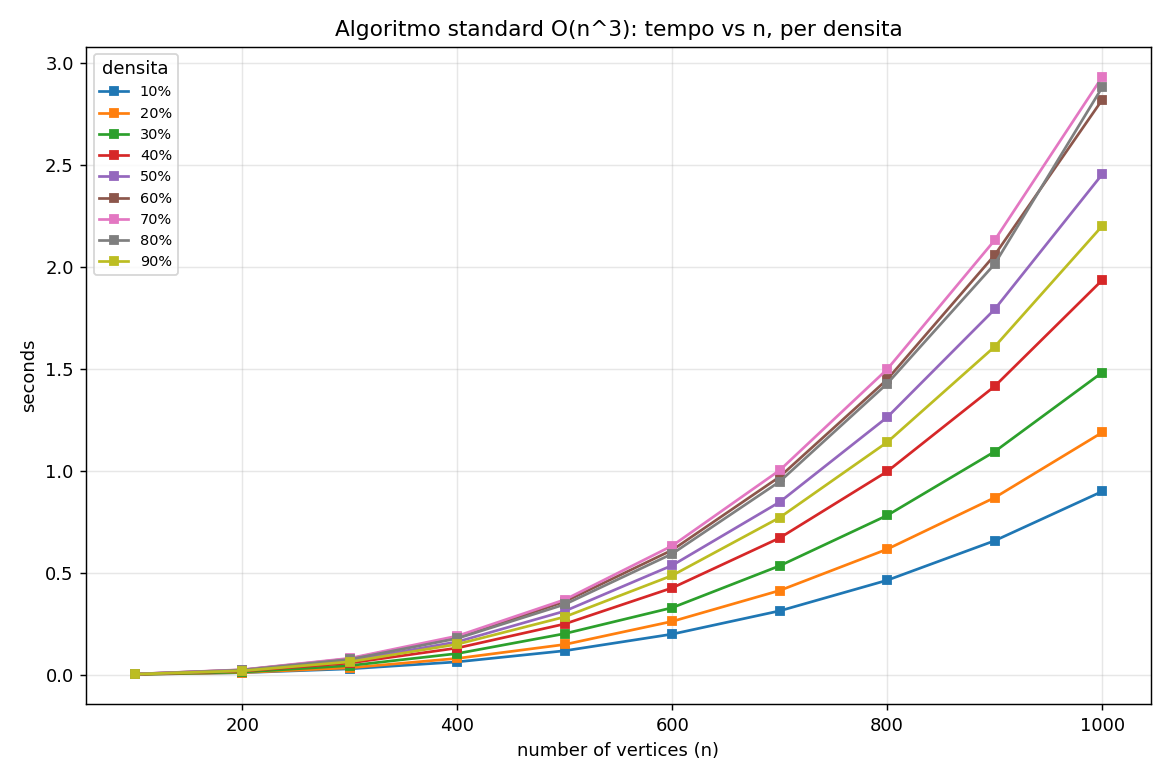
\includegraphics[width=0.8\textwidth]{standard_plot.png}
	\caption{Tempo di esecuzione dell'approccio standard $O(n^3)$ in funzione del
		numero di vertici, una curva per ciascuna densità.}
	\label{fig:standard}
\end{figure}

Il confronto diretto con l'algoritmo di Brandes (Figura~\ref{fig:confronto})
chiarisce dove stia il vantaggio. Sui grafi qui generati, a densità $10\%$--$90\%$,
si ha $m=\Theta(n^2)$: in questo regime denso anche Brandes costa $O(nm)=O(n^3)$, e
i tempi sono dunque dello stesso ordine (lo standard resta più lento per la
costante della somma esplicita). Il guadagno decisivo di Brandes emerge invece sui
grafi \emph{sparsi} --- tipici delle reti reali --- e, soprattutto, nello spazio:
$O(n+m)$ lineare contro $O(n^2)$.

\begin{figure}[H]
	\centering
	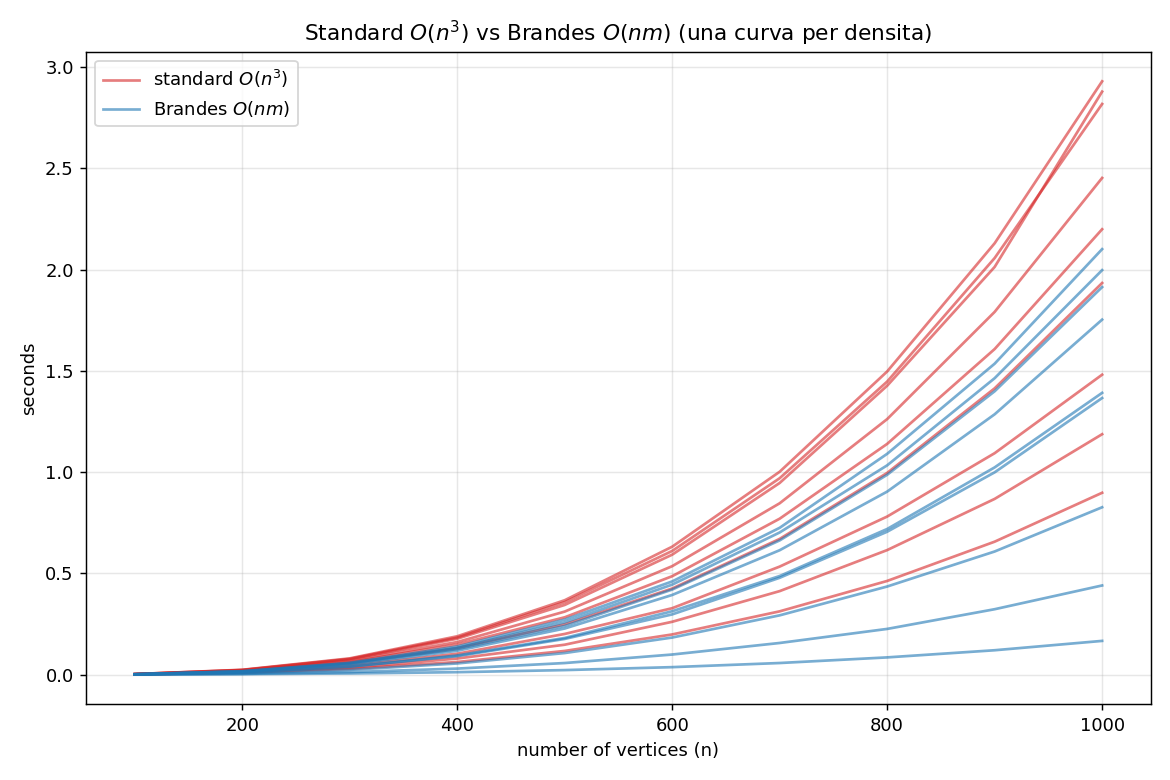
\includegraphics[width=0.8\textwidth]{confronto.png}
	\caption{Confronto dei tempi: approccio standard $O(n^3)$ (rosso) contro
		algoritmo di Brandes $O(nm)$ (blu), una curva per densità sul range di $n$
		comune.}
	\label{fig:confronto}
\end{figure}

\section{Il contributo di Brandes}

Nel 2001 Brandes~\cite{brandes2001} propone un algoritmo che riduce
sensibilmente il costo computazionale senza introdurre alcuna approssimazione.
L'idea centrale consiste nel non sommare le dipendenze coppia per coppia, bensì
nell'\emph{accumularle} in forma aggregata considerando una sola sorgente per
volta, attraverso una relazione ricorsiva sulle dipendenze discussa nel
Capitolo~2.

I costi ottenuti sono:
\begin{itemize}
	\item \textbf{grafi non pesati}: $O(nm)$ tempo, tramite una BFS
	      (\emph{Breadth-First Search}) da ciascuna sorgente;
	\item \textbf{grafi pesati}: $O(nm + n^2\log n)$ tempo, usando l'algoritmo di
	      Dijkstra con \emph{Fibonacci heap}~\cite{fredman1987};
	\item \textbf{spazio}: $O(n+m)$ in entrambi i casi, ovvero lineare.
\end{itemize}

La riduzione dello spazio da $O(n^2)$ a $O(n+m)$ è l'elemento che rende
l'algoritmo applicabile a reti di grande dimensione.

\section{Obiettivo}

La presente tesina documenta un'implementazione in C++ dell'algoritmo di Brandes
per grafi non orientati, ne verifica la correttezza mediante confronto con la
libreria NetworkX~\cite{networkx} e ne analizza sperimentalmente la complessità,
riproducendo lo schema di esperimento presentato nell'articolo originale. La
trattazione muove dal caso \emph{non pesato} (Capitolo~2), in cui i cammini minimi
sono determinati tramite la BFS, e si estende successivamente al
caso \emph{pesato} (Capitolo~3), in cui la costruzione dei cammini minimi è sostituita
dall'algoritmo di Dijkstra; di quest'ultima variante si illustrano il
funzionamento, le modifiche apportate al codice e l'andamento sperimentale dei
tempi di esecuzione al variare della densità.
Vengono inoltre discusse alcune ottimizzazioni a
costante (riutilizzo dei buffer di memoria) che, pur non modificando la
complessità asintotica $O(nm)$, riducono sensibilmente i tempi di esecuzione.


\chapter{Implementazione proposta}

Il presente capitolo descrive in dettaglio l'algoritmo di Brandes per grafi non
pesati, ponendo ciascun passo dello pseudocodice in corrispondenza con la
relativa porzione del codice C++ contenuto nel file \texttt{src/brandes.cpp}.

\section{La relazione ricorsiva sulle dipendenze}

Il fulcro dell'algoritmo è la nozione di \emph{dipendenza} di una sorgente $s$ da
un vertice $v$:
\begin{equation}
	\delta_s(v) = \sum_{t\in V} \frac{\sigma_{st}(v)}{\sigma_{st}}.
\end{equation}
Sommando $\delta_s(v)$ su tutte le sorgenti si riottiene
$C_B(v)=\sum_{s}\delta_s(v)$. Brandes dimostra che la dipendenza soddisfa la
relazione ricorsiva
\begin{equation}
	\delta_s(v) = \sum_{w\,:\,v\in P_s(w)}
	\frac{\sigma_{sv}}{\sigma_{sw}}\bigl(1+\delta_s(w)\bigr),
	\label{eq:ricorsione}
\end{equation}
dove $P_s(w)$ è l'insieme dei \emph{predecessori} di $w$ lungo i cammini minimi
da $s$, cioè i vertici $v$ adiacenti a $w$ tali che
$d(s,v)+1 = d(s,w)$.

È istruttivo soffermarsi sul fattore $\bigl(1+\delta_s(w)\bigr)$, che è il cuore
della relazione. Conviene però partire dal coefficiente
$\sigma_{sv}/\sigma_{sw}$. A numeratore $\sigma_{sv}$ è il numero di cammini
minimi da $s$ a $v$, a denominatore $\sigma_{sw}$ è il numero di cammini minimi
da $s$ a $w$ (non quelli che \emph{passano} per $w$, ma quelli che vi
\emph{arrivano}). Poiché $v$ è un predecessore di $w$, ogni cammino minimo da $s$
a $w$ che transita per $v$ si ottiene prolungando di un arco un cammino minimo da
$s$ a $v$: i cammini minimi verso $w$ passanti per $v$ sono dunque esattamente
$\sigma_{sv}$. Il rapporto $\sigma_{sv}/\sigma_{sw}$ è perciò la \emph{frazione}
dei cammini minimi diretti a $w$ che lo raggiungono passando per $v$, ovvero la
probabilità che, scelto a caso uno dei cammini minimi $s\to w$, esso transiti per
$v$. Non è quindi una misura di ``quanto $v$ dipende da $w$'', bensì la quota di
instradamento verso $w$ che spetta a $v$: è il peso con cui $v$ ha diritto a
ereditare la dipendenza di $w$. Questa frazione viene
moltiplicata per due contributi distinti. Il termine $1$ rappresenta la
dipendenza dovuta alla coppia $(s,w)$ \emph{stessa}: $v$ giace su un cammino
minimo da $s$ a $w$, dunque va accreditato come vertice intermedio rispetto alla
destinazione $w$. Il termine $\delta_s(w)$, invece, propaga a $v$ tutta la
dipendenza già accumulata da $w$: poiché $w$ sta sui cammini minimi verso ogni
destinazione $t$ \emph{più lontana di $w$}, e $v$ sta sui cammini minimi verso
$w$, allora $v$ giace anche su tutti i cammini minimi $s\to\dots\to v\to
w\to\dots\to t$. In altre parole, $v$ non viene accreditato soltanto per i
cammini che terminano in $w$, ma per ogni cammino minimo che parte da $s$, passa
per $v$ e per $w$, e prosegue oltre verso un qualunque vertice $t$ a valle di
$w$. È esattamente questa propagazione ricorsiva --- ogni successore $w$ cede a
$v$ la propria dipendenza più l'unità corrispondente a sé stesso come
destinazione --- che consente di evitare la somma esplicita coppia per coppia.

La relazione~\eqref{eq:ricorsione} permette quindi di calcolare
tutte le dipendenze di una sorgente con una sola passata all'indietro sui
vertici, in ordine di distanza non crescente.

\section{Dimostrazione della relazione ricorsiva}

La relazione~\eqref{eq:ricorsione} è il risultato centrale su cui poggia
l'algoritmo: ne giustifichiamo qui la validità, muovendo dalle definizioni di
base e appoggiandoci a due lemmi di natura combinatoria sui conteggi dei cammini
minimi. La dimostrazione segue quella originale di Brandes~\cite{brandes2001}.

\subsection*{Definizioni}

Per una coppia ordinata di vertici distinti $(s,t)$ si denotano con $\sigma_{st}$
il numero di cammini minimi da $s$ a $t$ e con $\sigma_{st}(v)$ il numero di
quelli che transitano per un vertice intermedio $v\neq s,t$; $d(s,t)$ è la
distanza fra $s$ e $t$. La \emph{betweenness centrality} di $v$ è
\begin{equation}
	C_B(v)=\sum_{s\neq v}\ \sum_{t\neq s,\,t\neq v}\frac{\sigma_{st}(v)}{\sigma_{st}},
	\label{eq:cb-def}
\end{equation}
e la quantità $\delta_{st}(v)=\sigma_{st}(v)/\sigma_{st}$, detta
\emph{dipendenza di coppia}, esprime la frazione dei cammini minimi $s\to t$ che
passano per $v$. Raggruppando i contributi a parità di sorgente si ottiene la
\emph{dipendenza} $\delta_s(v)=\sum_{t}\delta_{st}(v)$ già introdotta, per la
quale vale $C_B(v)=\sum_{s\neq v}\delta_s(v)$. Il calcolo diretto della
\eqref{eq:cb-def} richiederebbe di conoscere i $\Theta(n^3)$ valori
$\sigma_{st}(v)$; l'intera efficienza dell'algoritmo discende dal non calcolarli
mai esplicitamente, ma dal ricavare le dipendenze tramite la
\eqref{eq:ricorsione}.

Si chiama infine \emph{insieme dei predecessori} di $w$ rispetto a $s$
\[
	P_s(w)=\bigl\{\,u\in V : \{u,w\}\in E,\ d(s,w)=d(s,u)+1\,\bigr\},
\]
cioè l'insieme dei vertici da cui parte l'ultimo arco di un cammino minimo da $s$
a $w$; i predecessori inducono il \emph{grafo aciclico dei cammini minimi}
radicato in $s$.

\subsection*{Due lemmi sui conteggi}

\begin{lemma}[Conteggio dei cammini minimi]\label{lem:sigma}
	Per ogni $w\neq s$ vale $\displaystyle \sigma_{sw}=\sum_{u\in P_s(w)}\sigma_{su}$.
\end{lemma}
\begin{proof}
	\renewcommand{\qedsymbol}{}
	Ogni cammino minimo da $s$ a $w$ ha lunghezza $d(s,w)$ e termina con un arco
	$\{u,w\}$ tale che $d(s,u)=d(s,w)-1$, ossia $u\in P_s(w)$. Sopprimendone
	l'ultimo arco si ottiene un cammino minimo da $s$ a $u$, e tale operazione
	stabilisce una corrispondenza biunivoca fra i cammini minimi $s\to w$ aventi
	$u$ come penultimo vertice e i cammini minimi $s\to u$. Al variare di $u$ in
	$P_s(w)$ questi insiemi formano una partizione dei cammini minimi $s\to w$, da
	cui la somma.
\end{proof}

Il Lemma~\ref{lem:sigma} è esattamente la regola con cui la BFS aggiorna i
contatori $\sigma$: alla scoperta di un cammino minimo verso $w$ passante per $v$
si pone $\sigma[w]\mathrel{+}=\sigma[v]$.

\begin{lemma}[Fattorizzazione di un vertice intermedio]\label{lem:fattore}
	Se $v$ giace su almeno un cammino minimo da $s$ a $t$, allora
	$\sigma_{st}(v)=\sigma_{sv}\cdot\sigma_{vt}$.
\end{lemma}
\begin{proof}
	\renewcommand{\qedsymbol}{}
	Poiché $v$ è sul cammino minimo, $d(s,t)=d(s,v)+d(v,t)$: ogni cammino minimo
	$s\to t$ passante per $v$ si scompone in modo unico nella concatenazione di un
	cammino minimo $s\to v$ e di un cammino minimo $v\to t$. Viceversa, ogni coppia
	formata da un cammino minimo $s\to v$ e da un cammino minimo $v\to t$, accostata,
	dà un cammino minimo $s\to t$ passante per $v$. Il conteggio di un prodotto
	cartesiano è il prodotto dei conteggi.
\end{proof}

Dal Lemma~\ref{lem:fattore} segue immediatamente la forma esplicita della
dipendenza di coppia, $\delta_{st}(v)=\dfrac{\sigma_{sv}\,\sigma_{vt}}{\sigma_{st}}$.

\subsection*{Il teorema ricorsivo}

\begin{teorema}[Brandes, 2001]\label{th:ricorsione}
	Per ogni $v\neq s$ vale
	\[
		\delta_s(v)=\sum_{w\,:\,v\in P_s(w)}
		\frac{\sigma_{sv}}{\sigma_{sw}}\bigl(1+\delta_s(w)\bigr),
	\]
	dove la somma è estesa ai \emph{successori} di $v$ nel grafo dei cammini
	minimi, cioè ai vertici $w$ di cui $v$ è predecessore.
\end{teorema}
\begin{proof}
	\renewcommand{\qedsymbol}{}
	Si fissi $v\neq s$ e un bersaglio $t\neq s,v$. In ogni cammino minimo da $s$ a
	$t$ che passa per $v$, il vertice immediatamente successivo a $v$ è un vicino
	$w$ che ne è successore nel grafo dei cammini minimi, cioè $v\in P_s(w)$.
	Classificando tali cammini in base a questo primo vertice $w$ si ottiene una
	partizione, da cui
	\[
		\sigma_{st}(v)=\sum_{w\,:\,v\in P_s(w)}\sigma_{st}(v,w),
	\]
	avendo indicato con $\sigma_{st}(v,w)$ il numero di cammini minimi $s\to t$ che
	passano per $v$ e ne escono verso $w$.

	Questa quantità si fattorizza. Per $t\neq w$, un simile cammino è la
	concatenazione di un cammino minimo $s\to w$ avente $v$ come penultimo vertice
	con un cammino minimo $w\to t$; i primi sono $\sigma_{sv}$ (Lemma~\ref{lem:sigma},
	essendo $v\in P_s(w)$), sicché, usando $\sigma_{st}(w)=\sigma_{sw}\,\sigma_{wt}$
	(Lemma~\ref{lem:fattore}),
	\[
		\sigma_{st}(v,w)=\sigma_{sv}\,\sigma_{wt}=\frac{\sigma_{sv}}{\sigma_{sw}}\,\sigma_{st}(w).
	\]
	L'uguaglianza resta valida anche quando $w$ non giace su alcun cammino minimo
	$s\to t$: in tal caso $\sigma_{st}(w)=0$ ed entrambi i membri si annullano. Per
	$t=w$, infine, i cammini minimi $s\to w$ con penultimo vertice $v$ sono
	esattamente $\sigma_{sv}$, e il loro contributo a $\delta_s(v)$ è
	$\sigma_{sv}/\sigma_{sw}$.

	Sostituendo nella definizione di $\delta_s(v)$ e scambiando l'ordine delle
	somme,
	\[
		\delta_s(v)=\sum_{t\neq s,v}\frac{\sigma_{st}(v)}{\sigma_{st}}
		=\sum_{w\,:\,v\in P_s(w)}\Biggl(
		\underbrace{\frac{\sigma_{sv}}{\sigma_{sw}}}_{t=w}
		+\sum_{t\neq s,w}\frac{1}{\sigma_{st}}\cdot\frac{\sigma_{sv}}{\sigma_{sw}}\,\sigma_{st}(w)
		\Biggr).
	\]
	Nel secondo addendo si raccoglie il fattore costante e si riconosce la
	definizione di dipendenza:
	\[
		\frac{\sigma_{sv}}{\sigma_{sw}}\sum_{t\neq s,w}\frac{\sigma_{st}(w)}{\sigma_{st}}
		=\frac{\sigma_{sv}}{\sigma_{sw}}\,\delta_s(w).
	\]
	Sommando i due contributi relativi a ciascun successore $w$ si ottiene
	$\dfrac{\sigma_{sv}}{\sigma_{sw}}\bigl(1+\delta_s(w)\bigr)$ e, sommando su tutti
	i successori, la~\eqref{eq:ricorsione}.
\end{proof}

\subsection*{Conseguenza per l'algoritmo}

Nel Teorema~\ref{th:ricorsione} la dipendenza di $v$ è espressa in funzione delle
sole dipendenze $\delta_s(w)$ dei suoi successori, per i quali $d(s,w)>d(s,v)$. La
ricorsione è dunque \emph{ben fondata}: elaborando i vertici in ordine di distanza
non crescente, quando si tratta $v$ tutti i valori $\delta_s(w)$ necessari sono già
stati calcolati. È precisamente ciò che garantisce la pila $S$, che restituisce i
vertici nell'ordine inverso a quello di inserimento durante la BFS. L'algoritmo
realizza la somma ``per successori'' come una distribuzione ``ai predecessori'':
estratto $w$ da $S$, ne riversa il contributo
$\frac{\sigma_{sv}}{\sigma_{sw}}(1+\delta_s(w))$ su ciascun $v\in P_s(w)$.
Accumulando infine $C_B[w]\mathrel{+}=\delta_s(w)$ per ogni sorgente $s$, il vettore
$C_B$ riproduce esattamente la doppia somma~\eqref{eq:cb-def}; nel caso non
orientato ogni coppia non ordinata è conteggiata due volte, da cui la divisione
finale per $2$.

Vale la pena osservare che il calcolo delle dipendenze è, a tutti gli effetti, un
problema di \emph{programmazione dinamica}. Ne possiede infatti i due tratti
caratteristici: la \emph{sottostruttura ottima}, espressa dalla
relazione~\eqref{eq:ricorsione}, che riconduce $\delta_s(v)$ ai valori
$\delta_s(w)$ dei successori; e la \emph{sovrapposizione dei sottoproblemi},
poiché la dipendenza $\delta_s(w)$ di un vertice è condivisa da tutti i suoi
predecessori e dovrebbe essere ricalcolata molte volte se affrontata in modo
ingenuo. Risolvere ogni sottoproblema una sola volta e riutilizzarne il risultato
--- memorizzandolo nel vettore $\delta$ ed elaborando i vertici nell'ordine
topologico indotto dalla distanza decrescente (l'ordine di estrazione dalla pila
$S$) --- è esattamente ciò che trasforma la somma esplicita su tutte le coppie,
di costo $\Theta(n^3)$, nella passata lineare $O(m)$ per sorgente dell'algoritmo
di Brandes.

\begin{figure}[H]
	\centering
	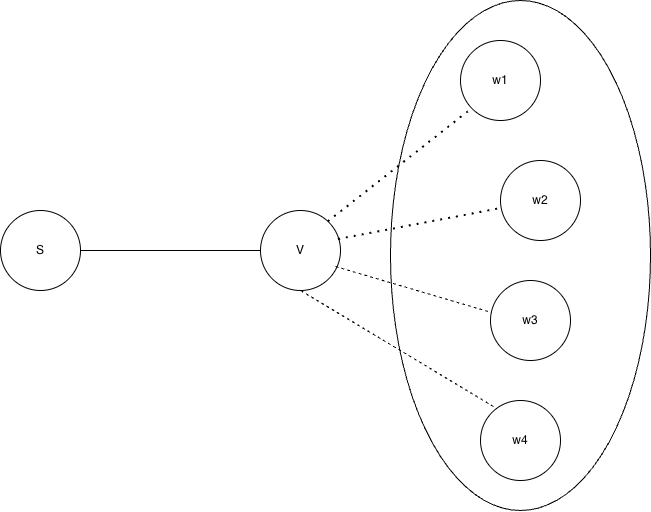
\includegraphics[width=0.75\textwidth]{dag_successori.png}
	\caption{Struttura locale del DAG dei cammini minimi attorno al nodo $v$. La
	sorgente $s$ raggiunge $v$ tramite i cammini minimi già processati; da $v$ si
	dipartono gli archi verso l'insieme dei successori
	$\{w_1,w_2,w_3,w_4\}=\{w:v\in P_s(w)\}$, cioè i nodi per cui $v$ è predecessore
	diretto nel DAG.}
	\label{fig:dag-successori}
\end{figure}

La Figura~\ref{fig:dag-successori} illustra la struttura locale sfruttata dalla
ricorsione nel calcolo della dipendenza $\delta_s(v)$. Fissata una sorgente $s$,
ogni cammino minimo che prosegue oltre $v$ verso un target più lontano deve
necessariamente transitare per uno dei successori di $v$ nel DAG dei cammini
minimi, qui indicati con $w_1,\dots,w_4$. Questi archi tratteggiati rappresentano
quindi una partizione dell'insieme dei target raggiungibili da $v$: ciascun target
lontano contribuisce alla dipendenza $\delta_s(v)$ attraverso esattamente uno di
questi successori. È questa proprietà a fondare la decomposizione
ricorsiva~\eqref{eq:ricorsione}; come osservato sopra, il contributo di ciascun
$w_i$ è già interamente noto al momento dell'elaborazione di $v$.

\clearpage
\section{Pseudocodice}

\begin{algorithm}[H]
	\caption{Betweenness centrality (Brandes, grafi non pesati)}
	\begin{algorithmic}[1]
		\State $C_B[v]\gets 0$ per ogni $v\in V$
		\For{$s\in V$}
		\State inizializza pila $S\gets\emptyset$, liste $P[w]\gets\emptyset$
		\State $\sigma[t]\gets 0$, $\sigma[s]\gets 1$
		\State $d[t]\gets -1$, $d[s]\gets 0$
		\State coda $Q\gets\{s\}$
		\While{$Q\neq\emptyset$} \Comment{BFS}
		\State estrai $v$ da $Q$; inserisci $v$ in $S$
		\For{ogni vicino $w$ di $v$}
		\If{$d[w]<0$} \Comment{$w$ trovato per la prima volta}
		\State $d[w]\gets d[v]+1$; inserisci $w$ in $Q$
		\EndIf
		\If{$d[w]=d[v]+1$} \Comment{cammino minimo verso $w$ via $v$}
		\State $\sigma[w]\gets\sigma[w]+\sigma[v]$
		\State inserisci $v$ in $P[w]$
		\EndIf
		\EndFor
		\EndWhile
		\State $\delta[v]\gets 0$ per ogni $v$
		\While{$S\neq\emptyset$} \Comment{accumulo all'indietro}
		\State estrai $w$ dalla cima di $S$
		\For{ogni $v\in P[w]$}
		\State $\delta[v]\gets\delta[v]+\frac{\sigma[v]}{\sigma[w]}(1+\delta[w])$
		\EndFor
		\If{$w\neq s$} $C_B[w]\gets C_B[w]+\delta[w]$ \EndIf
		\EndWhile
		\EndFor
		\State \textbf{per grafi non orientati:} $C_B[v]\gets C_B[v]/2$ per ogni $v$
	\end{algorithmic}
\end{algorithm}

\section{Esempio passo-passo: il diamante a 5 vertici}

Per rendere concreto lo pseudocodice si segue l'esecuzione dell'algoritmo su un
piccolo grafo non pesato, mostrando l'evoluzione di tutti i vettori coinvolti. Si
considera il grafo di Figura~\ref{fig:diamante}, con $n=5$ vertici e gli archi
\[
	\{0,1\},\ \{0,2\},\ \{1,3\},\ \{2,3\},\ \{3,4\}.
\]
La struttura a diamante fra $0$, $1$, $2$, $3$ è scelta deliberatamente: da $0$ a
$3$ esistono \emph{due} cammini minimi, $0\!-\!1\!-\!3$ e $0\!-\!2\!-\!3$, così da
osservare il conteggio $\sigma$ assumere un valore maggiore di $1$.

\begin{figure}[H]
	\centering
	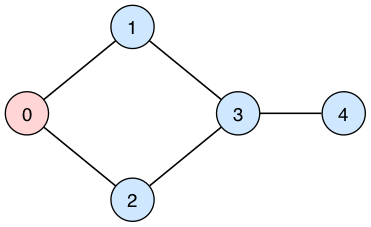
\includegraphics[width=0.5\textwidth]{diamante.png}
	\caption{Il diamante a $5$ vertici. In rosso la sorgente $s=0$ da cui si avvia
		la visita.}
	\label{fig:diamante}
\end{figure}

\subsection*{Fase 1: il calcolo dei cammini minimi dalla sorgente $s=0$}

All'avvio $d[0]=0$, $\sigma[0]=1$, mentre per ogni altro vertice $d=-1$ (non
visitato) e $\sigma=0$; la coda contiene $\{0\}$. Le due tabelle seguenti
riportano lo stato \emph{successivo} all'estrazione di ciascun nodo dalla coda
(il valore $-1$ indica un vertice non ancora raggiunto).

\begin{table}[H]
	\centering
	\caption{Evoluzione di \texttt{d} (calcolo dei cammini minimi da $s=0$).}
	\begin{tabular}{l rrrrr}
		\toprule
		nodo estratto & $d_0$ & $d_1$ & $d_2$ & $d_3$ & $d_4$ \\
		\midrule
		-- init --    & 0     & $-1$  & $-1$  & $-1$  & $-1$  \\
		0             & 0     & 1     & 1     & $-1$  & $-1$  \\
		1             & 0     & 1     & 1     & 2     & $-1$  \\
		2             & 0     & 1     & 1     & 2     & $-1$  \\
		3             & 0     & 1     & 1     & 2     & 3     \\
		4             & 0     & 1     & 1     & 2     & 3     \\
		\bottomrule
	\end{tabular}
\end{table}

\begin{table}[H]
	\centering
	\caption{Evoluzione di \texttt{sigma} (numero di cammini minimi).}
	\begin{tabular}{l rrrrr}
		\toprule
		nodo estratto & $\sigma_0$ & $\sigma_1$ & $\sigma_2$ & $\sigma_3$ & $\sigma_4$ \\
		\midrule
		-- init --    & 1          & 0          & 0          & 0          & 0          \\
		0             & 1          & 1          & 1          & 0          & 0          \\
		1             & 1          & 1          & 1          & 1          & 0          \\
		2             & 1          & 1          & 1          & \textbf{2} & 0          \\
		3             & 1          & 1          & 1          & 2          & 2          \\
		4             & 1          & 1          & 1          & 2          & 2          \\
		\bottomrule
	\end{tabular}
\end{table}

Il passaggio cruciale è l'estrazione del nodo $2$: poiché $d_3 = d_2+1$, il nodo
$3$ riceve un \emph{secondo} contributo e $\sigma_3$ passa da $1$ a $2$, in
corrispondenza dei due cammini minimi del diamante. Tale valore $2$ si propaga
poi al nodo $4$. Al termine della visita la pila \texttt{S} contiene (dal fondo
alla cima)
\[
	\texttt{S} = [\,0,\ 1,\ 2,\ 3,\ 4\,].
\]

\subsubsection*{Evoluzione di \texttt{Q} e \texttt{S}}

Le due strutture hanno ruoli complementari: la coda \texttt{Q} guida l'\emph{ordine
di scoperta} dei vertici, mentre la pila \texttt{S} ne \emph{registra} l'ordine di
visita per poterlo poi ripercorrere a ritroso nella fase di accumulo. La
Tabella~\ref{tab:qs} ne mostra l'evoluzione congiunta: a ogni passo si estrae un
vertice $v$ dalla testa di \texttt{Q}, lo si inserisce in \texttt{S} e si
aggiungono in coda a \texttt{Q} i soli vicini non ancora scoperti (quelli con
$d=-1$). In tal modo ciascun vertice entra in \texttt{Q} una sola volta.

\begin{table}[H]
	\centering
	\caption{Evoluzione di \texttt{Q} (coda FIFO) e \texttt{S} (pila) durante la
		visita da $s=0$.}
	\label{tab:qs}
	\begin{tabular}{l l l l}
		\toprule
		$v$ estratto & vicini nuovi $\to$ \texttt{Q} & \texttt{Q} (testa$\to$coda) & \texttt{S} (fondo$\to$cima) \\
		\midrule
		-- init -- & $0$     & $[\,0\,]$       & $[\,\,]$            \\
		$0$        & $1,\ 2$ & $[\,1,2\,]$     & $[\,0\,]$           \\
		$1$        & $3$     & $[\,2,3\,]$     & $[\,0,1\,]$         \\
		$2$        & --      & $[\,3\,]$       & $[\,0,1,2\,]$       \\
		$3$        & $4$     & $[\,4\,]$       & $[\,0,1,2,3\,]$     \\
		$4$        & --      & $[\,\,]$        & $[\,0,1,2,3,4\,]$   \\
		\bottomrule
	\end{tabular}
\end{table}

Si nota come \texttt{Q} si riempia e si svuoti \emph{contestualmente} (a ogni
estrazione corrispondono zero o più inserimenti dei vicini nuovi), fino a
svuotarsi del tutto a visita conclusa; \texttt{S}, invece, si riempie soltanto,
accumulando i vertici in ordine di distanza crescente. La fase di accumulo,
descritta nel seguito, svuota poi \texttt{S} estraendo dalla cima: l'ordine
risultante $4,3,2,1,0$ è quello a distanza \emph{decrescente}, esattamente come
richiesto dalla relazione ricorsiva. È questa la ragione per cui si impiega una
pila e non una seconda coda: la struttura LIFO inverte automaticamente l'ordine
di visita.

\subsection*{Fase 2: accumulo delle dipendenze}

Si svuota la pila \texttt{S} estraendo i nodi dalla cima (da $4$ a $0$). Per ogni nodo $w$ si
aggiornano i suoi predecessori $v$, quelli con $d_v = d_w-1$, mediante
\[
	\delta_v \mathrel{+}= \frac{\sigma_v}{\sigma_w}\,(1+\delta_w).
\]

\begin{table}[H]
	\centering
	\caption{Evoluzione di \texttt{delta} durante l'accumulo all'indietro ($s=0$).}
	\begin{tabular}{l rrrrr}
		\toprule
		$w$ corrente & $\delta_0$ & $\delta_1$ & $\delta_2$ & $\delta_3$ & $\delta_4$ \\
		\midrule
		(start)      & 0          & 0          & 0          & 0          & 0          \\
		4            & 0          & 0          & 0          & 1          & 0          \\
		3            & 0          & 1          & 1          & 1          & 0          \\
		2            & 2          & 1          & 1          & 1          & 0          \\
		1            & 4          & 1          & 1          & 1          & 0          \\
		\bottomrule
	\end{tabular}
\end{table}

Dettaglio dei passaggi più significativi:
\begin{itemize}
	\item \textbf{$w=4$}: unico predecessore $3$; $\delta_3 \mathrel{+}=
		      \frac{\sigma_3}{\sigma_4}(1+\delta_4)=\frac{2}{2}(1+0)=1$.
	\item \textbf{$w=3$}: due predecessori, $1$ e $2$; ciascuno riceve
	      $\frac{\sigma_v}{\sigma_3}(1+\delta_3)=\frac{1}{2}(1+1)=1$. Qui la
	      dipendenza si ripartisce fra i due cammini minimi alternativi.
	\item \textbf{$w=2$} e \textbf{$w=1$}: il predecessore è la sorgente $0$;
	      ognuno aggiunge $\frac{1}{1}(1+1)=2$, portando $\delta_0$ a $4$.
\end{itemize}

L'ultima estrazione, quella della sorgente $0$, è omessa dalla tabella perché non
produce alcun aggiornamento: la sorgente non ha predecessori (nessun vertice $v$
con $d_v = d_0-1 = -1$) e la sua dipendenza $\delta_0$ non viene comunque sommata a
$C_B$, in quanto $w=s$. Il contributo della sola sorgente $s=0$ è quindi
\[
	C_B^{(s=0)} = [\,0,\ 1,\ 1,\ 1,\ 0\,].
\]

\subsection*{Risultato finale}

Ripetendo la procedura per tutte le sorgenti $s=0,\dots,4$, sommando i contributi
e dividendo per $2$ (grafo non orientato) si ottiene
\[
	C_B = [\,0.5,\ 1.0,\ 1.0,\ 3.5,\ 0.0\,].
\]
Il nodo $3$ presenta la betweenness nettamente maggiore: è il \emph{ponte} del
grafo, attraversato dalla quasi totalità dei cammini minimi. I nodi $1$ e $2$,
simmetrici, hanno valore identico, mentre il nodo $4$, foglia, ha betweenness
nulla.

\section{Generazione dei grafi di test}

Le prove sperimentali richiedono la generazione di grafi casuali \emph{connessi}:
un grafo disconnesso falserebbe l'analisi dei tempi, in quanto il calcolo dei
cammini minimi da una data sorgente esplorerebbe la sola componente cui essa appartiene.
La funzione \texttt{genera\_grafo} costruisce dapprima uno \emph{spanning tree}
casuale, che garantisce la connessione mediante $n-1$ archi, e aggiunge
successivamente archi casuali fino a raggiungere il numero $m$ richiesto,
escludendo cappi e archi multipli.

\begin{lstlisting}[caption={Generazione di un grafo connesso (estratto).}]
// 1) spanning tree casuale: ogni nodo i si collega a un nodo precedente
for (int i = 1; i < n; i++) {
  std::uniform_int_distribution<int> prec(0, i - 1);
  aggiungi(i, prec(gen));
}
// 2) archi restanti scelti a caso fino a m archi totali
std::uniform_int_distribution<int> dist(0, n - 1);
while ((int)g.U.size() < m) {
  aggiungi(dist(gen), dist(gen));
}
\end{lstlisting}

La lambda \texttt{aggiungi} normalizza l'arco $(u,v)$ con $u<v$, scarta i
duplicati tramite un \texttt{std::set} e aggiorna le liste di adiacenza.

\section{Il calcolo dei cammini minimi}

Il blocco che realizza il calcolo dei cammini minimi determina, per ciascun
vertice, la distanza \texttt{d} e il numero di cammini minimi \texttt{sigma}, e
inserisce i vertici nell'ordine di visita nella pila \texttt{S} (la pila $S$ dello
pseudocodice). La coda dei nodi ancora da espandere è chiamata \texttt{Q}.
Si osserva la piena corrispondenza con le righe 7--14 dello pseudocodice.

Per la pila $S$ si è scelto \texttt{std::stack}, che corrisponde direttamente alla
struttura dello pseudocodice. Una soluzione equivalente sarebbe un \texttt{std::vector}
riempito durante la visita e percorso all'indietro: le due realizzazioni hanno la
stessa complessità e, in pratica, prestazioni indistinguibili; si è preferito
\texttt{std::stack} per la maggiore aderenza all'algoritmo descritto.

\begin{lstlisting}[caption={Calcolo dei cammini minimi con il relativo conteggio (BFS).}]
while (!Q.empty()) {
  int v = Q.front();
  Q.pop();
  S.push(v);                          // inserimento nella pila
  for (int w : g.adj[v]) {
    if (d[w] == -1) {                 // primo ritrovamento
      d[w] = d[v] + 1;
      Q.push(w);
    }
    if (d[w] == d[v] + 1)             // cammino minimo verso w
      sigma[w] += sigma[v];
  }
}
\end{lstlisting}

Il vettore \texttt{sigma} è dichiarato di tipo \texttt{long long}: su grafi di
grandi dimensioni ed elevata densità il numero di cammini minimi può eccedere
l'intervallo rappresentabile da \texttt{int}, e tale scelta previene l'overflow.

\section{L'accumulo all'indietro}

Terminato il calcolo dei cammini minimi, i vertici vengono esaminati in ordine di
distanza non crescente --- estraendoli dalla pila \texttt{S} --- e
si applica la relazione~\eqref{eq:ricorsione}. Una scelta implementativa
rilevante consiste nel \emph{non} memorizzare esplicitamente le liste dei
predecessori $P[w]$: poiché un vicino $v$ di $w$ ne è predecessore se e solo se
$d[v]=d[w]-1$, i predecessori sono ricalcolati direttamente a partire dal solo
vettore \texttt{d}, evitando l'occupazione di memoria e le numerose
allocazioni dinamiche che la gestione esplicita di $P[w]$ comporterebbe.

\begin{lstlisting}[caption={Accumulo delle dipendenze (predecessori ricalcolati).}]
while (!S.empty()) {
  int w = S.top();
  S.pop();
  for (int v : g.adj[w]) {
    if (d[v] == d[w] - 1)               // v e' predecessore di w
      delta[v] += (double)sigma[v] / sigma[w] * (1 + delta[w]);
  }
  if (w != s)
    CB[w] += delta[w];
}
\end{lstlisting}

Al termine del ciclo su tutte le sorgenti, trattandosi di un grafo non
orientato, ciascuna coppia risulta conteggiata due volte; il valore $C_B[v]$
viene pertanto diviso per $2$.

\section{Ottimizzazioni implementative}

L'implementazione adotta alcune ottimizzazioni che, pur lasciando invariata la
complessità asintotica $O(nm)$, ne riducono la costante moltiplicativa:
\begin{itemize}
	\item i buffer \texttt{d}, \texttt{sigma} e \texttt{delta}
	      sono allocati \emph{una sola volta} all'esterno del ciclo sulle sorgenti
	      e, a ogni iterazione, vengono riscritti tramite \texttt{std::fill}
	      anziché riallocati; analogamente la pila \texttt{S} è dichiarata una sola
	      volta e riutilizzata, poiché la fase di accumulo la svuota completamente
	      a fine sorgente. Ciò elimina $n$ coppie di operazioni
	      \texttt{malloc}/\texttt{free} per esecuzione;
	\item l'eliminazione delle liste di predecessori $P[w]$, illustrata in
	      precedenza, rimuove l'allocazione dinamica più onerosa dell'algoritmo;
	\item per la frontiera della BFS si è mantenuto
	      \texttt{std::queue} (basato su \texttt{std::deque}). È stata valutata
	      l'alternativa di una coda FIFO ad array preallocato con due indici, che
	      eviterebbe le allocazioni a blocchi del \texttt{deque}; il confronto
	      sperimentale non ha però evidenziato alcun guadagno (con
	      l'ottimizzazione \texttt{-O2} il \texttt{deque} riusa i blocchi già
	      allocati tra una sorgente e l'altra). Si è perciò preferito
	      \texttt{std::queue} per la maggiore leggibilità;
	\item prima delle misurazioni viene eseguita una breve fase di
	      \emph{warm-up} --- alcune esecuzioni preliminari su un grafo di dimensione
	      intermedia, i cui risultati sono scartati --- al fine di portare il
	      processore alla frequenza di regime e di precaricare le memorie cache,
	      attenuando l'artefatto di misura noto come ``primo punto lento''.
\end{itemize}
Come mostrato nel Capitolo~4, l'output numerico rimane identico a quello della
versione non ottimizzata, a meno del rumore in virgola mobile.

\subsection{Rappresentazione dell'adiacenza: liste contro CSR}

La rappresentazione adottata per le liste di adiacenza è un vettore di vettori
(\texttt{std::vector<std::vector<int>>}): assimilabile a una matrice irregolare
in cui ogni riga corrisponde a un vertice e gli elementi della riga sono i suoi
vicini. Ciascuna riga è però un blocco di memoria allocato separatamente, e
quindi potenzialmente lontano dagli altri: la scansione dei vicini durante la BFS
comporta un salto verso un'area di memoria scollegata, con possibili
\emph{cache miss}.

Si è perciò valutata una rappresentazione alternativa, il formato
\emph{Compressed Sparse Row} (CSR), che sostituisce il vettore di vettori con due
soli array contigui: un array \texttt{adj} che contiene tutti i vicini
concatenati in un unico blocco, e un array \texttt{offset} che, per ciascun
vertice $v$, individua l'intervallo di \texttt{adj} corrispondente ai suoi vicini
(da \texttt{offset[$v$]} a \texttt{offset[$v+1$]$-1$}). L'intera adiacenza occupa
così una sola zona di memoria, percorsa in modo sequenziale e prevedibile dal
\emph{prefetcher} hardware.

Sul piano teorico la CSR dovrebbe ridurre i \emph{cache miss}, con vantaggio
crescente sui grafi densi, dove la scansione dei vicini domina il costo. Il
confronto sperimentale --- a parità di algoritmo, cambiando unicamente la
rappresentazione --- non ha però evidenziato alcun guadagno misurabile: come
mostrato in Figura~\ref{fig:confronto-csr}, le due curve risultano sostanzialmente
sovrapposte a ogni densità, con un rapporto medio dei tempi compreso tra
$0{,}96$ e $1{,}01$. La ragione più plausibile è che l'ottimizzazione del
compilatore (\texttt{-O3}) e il riuso dei blocchi di memoria già allocati tra una
sorgente e l'altra rendano di fatto irrilevante la differenza di layout: il
sistema di memoria sottostante riesce già a servire con efficienza anche
l'accesso al vettore di vettori. Si tratta dunque di un'ottimizzazione
\emph{ipotizzata e sperimentalmente smentita}, analogamente a quanto osservato
per la coda della BFS.

\begin{figure}[h]
	\centering
	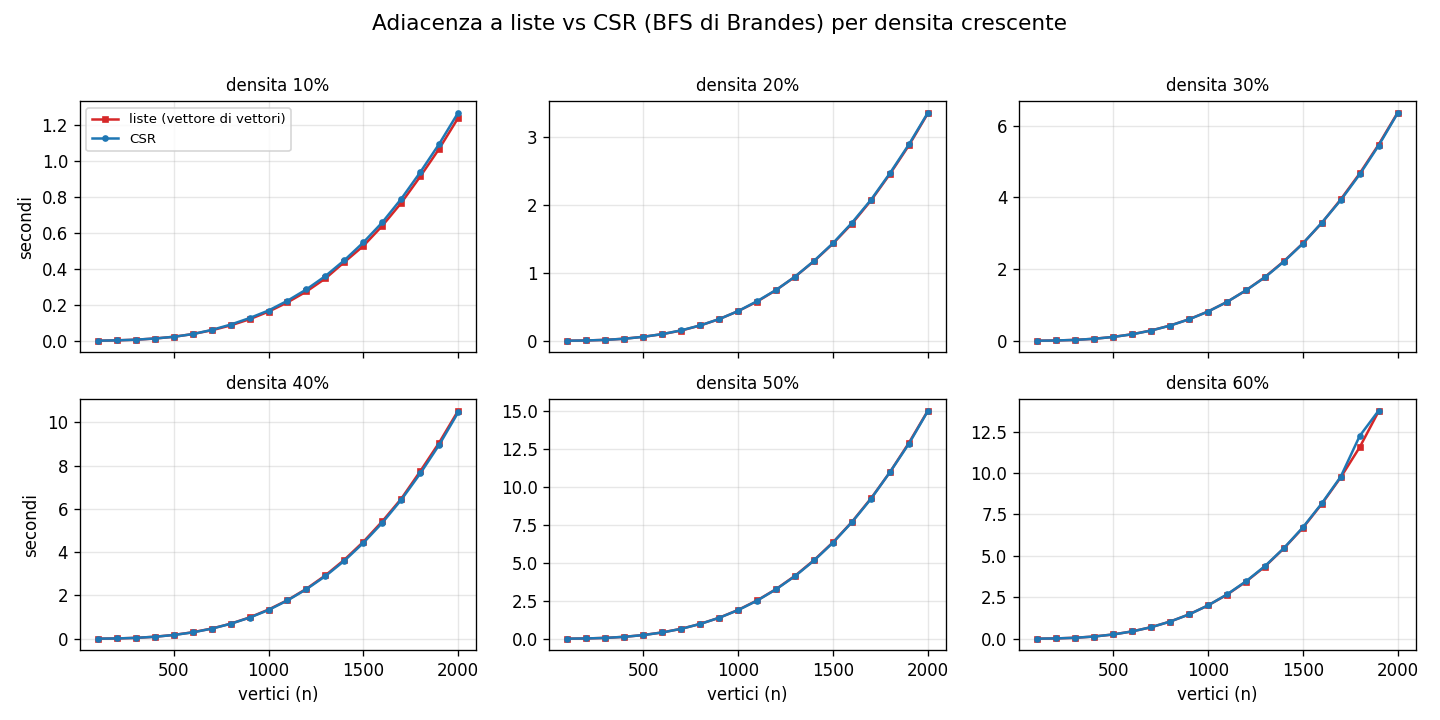
\includegraphics[width=\textwidth]{confronto_csr.png}
	\caption{Tempo di esecuzione della BFS di Brandes con adiacenza a liste
		(vettore di vettori) e in formato CSR, per densità crescente. Le curve
		sono sostanzialmente sovrapposte: la CSR non porta un guadagno
		misurabile.}
	\label{fig:confronto-csr}
\end{figure}


\chapter{Estensione ai grafi pesati: l'algoritmo di Dijkstra}

Quanto esposto finora si riferisce a grafi \emph{non pesati}, in cui ogni arco ha
costo unitario. In numerose applicazioni reali, tuttavia, agli archi è associato
un peso, interpretabile come distanza, tempo o capacità. Il presente capitolo
descrive come l'algoritmo di Brandes debba essere modificato per trattare i grafi
pesati; la corrispondente implementazione è contenuta nel file
\texttt{src/brandes\_weighted.cpp}.

\section{Inadeguatezza della BFS}

La BFS determina correttamente i cammini minimi soltanto quando
tutti gli archi hanno costo identico: in tal caso il primo istante in cui un
vertice viene raggiunto corrisponde al suo cammino minimo, e il numero di archi
coincide con la distanza. In presenza di pesi questa proprietà decade, poiché un
cammino composto da più archi di peso ridotto può risultare complessivamente più
breve di un singolo arco di peso elevato. La BFS, che procede per
livelli di numero di archi, non individuerebbe tali cammini.

La struttura generale dell'algoritmo di Brandes --- elaborazione di una sorgente
per volta, con una fase di calcolo dei cammini minimi seguita dall'accumulo
all'indietro delle dipendenze --- rimane invariata: a mutare è esclusivamente la
prima fase, in cui la BFS è sostituita dall'algoritmo di
\textbf{Dijkstra}. La relazione ricorsiva sulle dipendenze e la fase di accumulo
conservano la medesima logica.

\section{Implementazione con pesi non unitari}

Rispetto alla versione non pesata si rendono necessarie tre modifiche.

\paragraph{1. Calcolo delle distanze.} Il vettore \texttt{d}
assume tipo \texttt{long long}, dovendo accumulare la somma dei pesi anziché un
conteggio di livelli, ed è inizializzato a $+\infty$ in luogo di $-1$; il valore
infinito è rappresentato dal massimo valore esprimibile dal tipo.

\paragraph{2. Coda a priorità in luogo della coda FIFO.} La \texttt{std::queue} è
sostituita da una \texttt{std::priority\_queue} configurata come \emph{min-heap}:
in cima si trova costantemente il vertice di distanza provvisoria minima, ossia il
successivo da finalizzare. Il modificatore \texttt{std::greater} inverte
l'ordinamento predefinito --- che fornirebbe il massimo --- restituendo il minimo.

\paragraph{3. Azzeramento di \texttt{sigma} alla scoperta di cammini più brevi.}
Quando si individua un cammino \emph{strettamente} più breve verso un vicino, i
conteggi di cammini minimi accumulati fino a quel momento si riferiscono a una
distanza ormai superata e perdono validità; il valore \texttt{sigma[w]} viene
pertanto azzerato prima di riavviare il conteggio.

\begin{lstlisting}[caption={Fase 1 pesata: Dijkstra con conteggio dei cammini
minimi.}]
while (!Q.empty()) {
  auto [dv, v] = Q.top();              // dv: chiave estratta, ignorata
  Q.pop();
  if (nodi_completati[v]) continue;    // voce obsoleta: scarta
  nodi_completati[v] = 1;
  S.push(v);
  for (auto [w, peso] : g.adj[v]) {
    long long nd = d[v] + peso;
    if (nd < d[w]) {                   // cammino piu' corto
      d[w] = nd;
      sigma[w] = 0;                    // i conteggi vecchi non sono piu' minimi
      Q.push({nd, w});
    }
    if (nd == d[w])                    // altro cammino minimo verso w
      sigma[w] += sigma[v];
  }
}
\end{lstlisting}

\section{La cancellazione pigra}

La \texttt{std::priority\_queue} della libreria standard non mette a disposizione
l'operazione di \emph{decrease-key}, ossia l'aggiornamento della priorità di un
elemento già inserito. Si ricorre pertanto alla tecnica della \emph{cancellazione
	pigra} (\emph{lazy deletion}): all'individuazione di una distanza migliore per un
vertice si inserisce una nuova coppia $(d,\text{vertice})$, lasciando inalterata
la voce precedente. Al momento dell'estrazione, qualora il vertice risulti già
finalizzato (in base al flag \texttt{nodi\_completati}), la voce è obsoleta e viene scartata
mediante \texttt{continue}. In tal modo ciascun vertice è inserito nella pila
\texttt{S} una sola volta, secondo l'ordine di distanza crescente,
indispensabile per la successiva fase di accumulo.

La correttezza di questo schema --- finalizzare un vertice alla sua \emph{prima}
estrazione e scartare le copie successive --- è dovuta appunto
dal min-heap: nel momento in cui un vertice $v$ viene estratto per la
prima volta, la sua distanza provvisoria è \emph{già} quella minima definitiva, e
nessun cammino più breve potrà essere scoperto in seguito.
Si osservi che questa proprietà dipende in modo essenziale dall'ipotesi di
\textbf{pesi non negativi}: con archi di peso negativo un cammino più breve
potrebbe emergere \emph{dopo} la finalizzazione di un vertice, e l'algoritmo di
Dijkstra --- cancellazione pigra inclusa --- fornirebbe risultati errati. È
precisamente per questo motivo che Dijkstra richiede pesi non negativi; in
presenza di pesi negativi occorre ricorrere ad algoritmi diversi, come quello di
Bellman--Ford.

\section{L'accumulo all'indietro nel caso pesato}

La fase di accumulo è strutturalmente identica a quella del caso non pesato: i
vertici sono estratti dalla pila \texttt{S} e la dipendenza è distribuita ai
predecessori. L'unica differenza risiede nella \emph{condizione di predecessore}:
nel caso non pesato un vicino $v$ di $w$ ne è predecessore se $d_v = d_w - 1$,
mentre nel caso pesato la condizione diviene
\begin{equation}
	d_v + \text{peso}(v,w) = d_w .
\end{equation}
Analogamente al caso non pesato, i predecessori sono ricalcolati a partire dalle
distanze, senza il mantenimento di liste esplicite.

\noindent\begin{minipage}{\linewidth}
	\begin{lstlisting}[caption={Accumulo pesato: cambia solo la condizione di
predecessore.}]
while (!S.empty()) {
  int w = S.top();
  S.pop();
  for (auto [v, peso] : g.adj[w])
    if (d[v] + peso == d[w])          // v e' predecessore di w
      delta[v] += (double)sigma[v] / sigma[w] * (1 + delta[w]);
  if (w != s) CB[w] += delta[w];
}
\end{lstlisting}
\end{minipage}

\section{Complessità}

Con la coda a priorità l'estrazione del minimo e l'inserimento hanno costo
$O(\log n)$ ciascuno e si effettuano $O(m)$ aggiornamenti per sorgente; la singola
esecuzione di Dijkstra costa pertanto $O(m\log n)$, a fronte dell'$O(m)$ della
BFS. Esteso a tutte le $n$ sorgenti, il costo complessivo risulta
\begin{equation}
	O\bigl(nm\log n\bigr)
\end{equation}
nel caso di heap binario. L'impiego di un \emph{Fibonacci heap}~\cite{fredman1987},
che ammortizza l'operazione di \emph{decrease-key} a $O(1)$, consente di
raggiungere il costo teorico $O(nm + n^2\log n)$ indicato da Brandes.
Il fattore logaritmico aggiuntivo rappresenta il costo della maggiore generalità:
il caso pesato è intrinsecamente più oneroso di quello non pesato. La
Figura~\ref{fig:tempi_w} riporta i tempi misurati per la versione pesata, secondo
lo stesso schema sperimentale adottato nel caso non pesato --- una curva per
ciascuna densità, con sweep su $n$ ---; l'andamento conferma il maggiore costo
imputabile alla coda a priorità.

\begin{figure}[H]
	\centering
	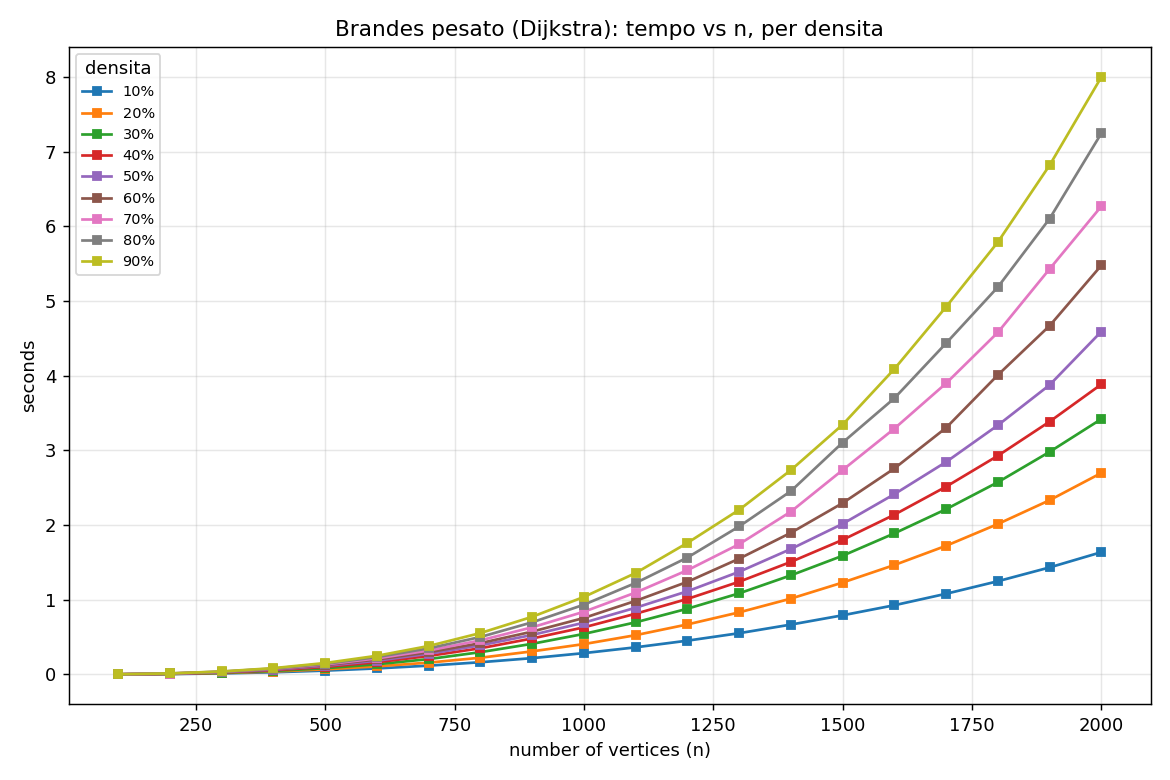
\includegraphics[width=0.8\textwidth]{brandes_plot_w.png}
	\caption{Tempo di esecuzione della versione pesata (Dijkstra) in funzione del
		numero di vertici, una curva per ciascuna densità.}
	\label{fig:tempi_w}
\end{figure}

\section{Verifica ed esempio visivo}

Anche la versione pesata è stata validata mediante confronto dei valori di $C_B$
con quelli prodotti da NetworkX, invocata con l'opzione \texttt{weight='weight'}
oltre a \texttt{normalized=False}: i risultati coincidono. La
Figura~\ref{fig:grafo_w} riporta un grafo pesato di esempio con i nodi-ponte
evidenziati; le etichette sugli archi ne indicano i pesi.

\begin{figure}[H]
	\centering
	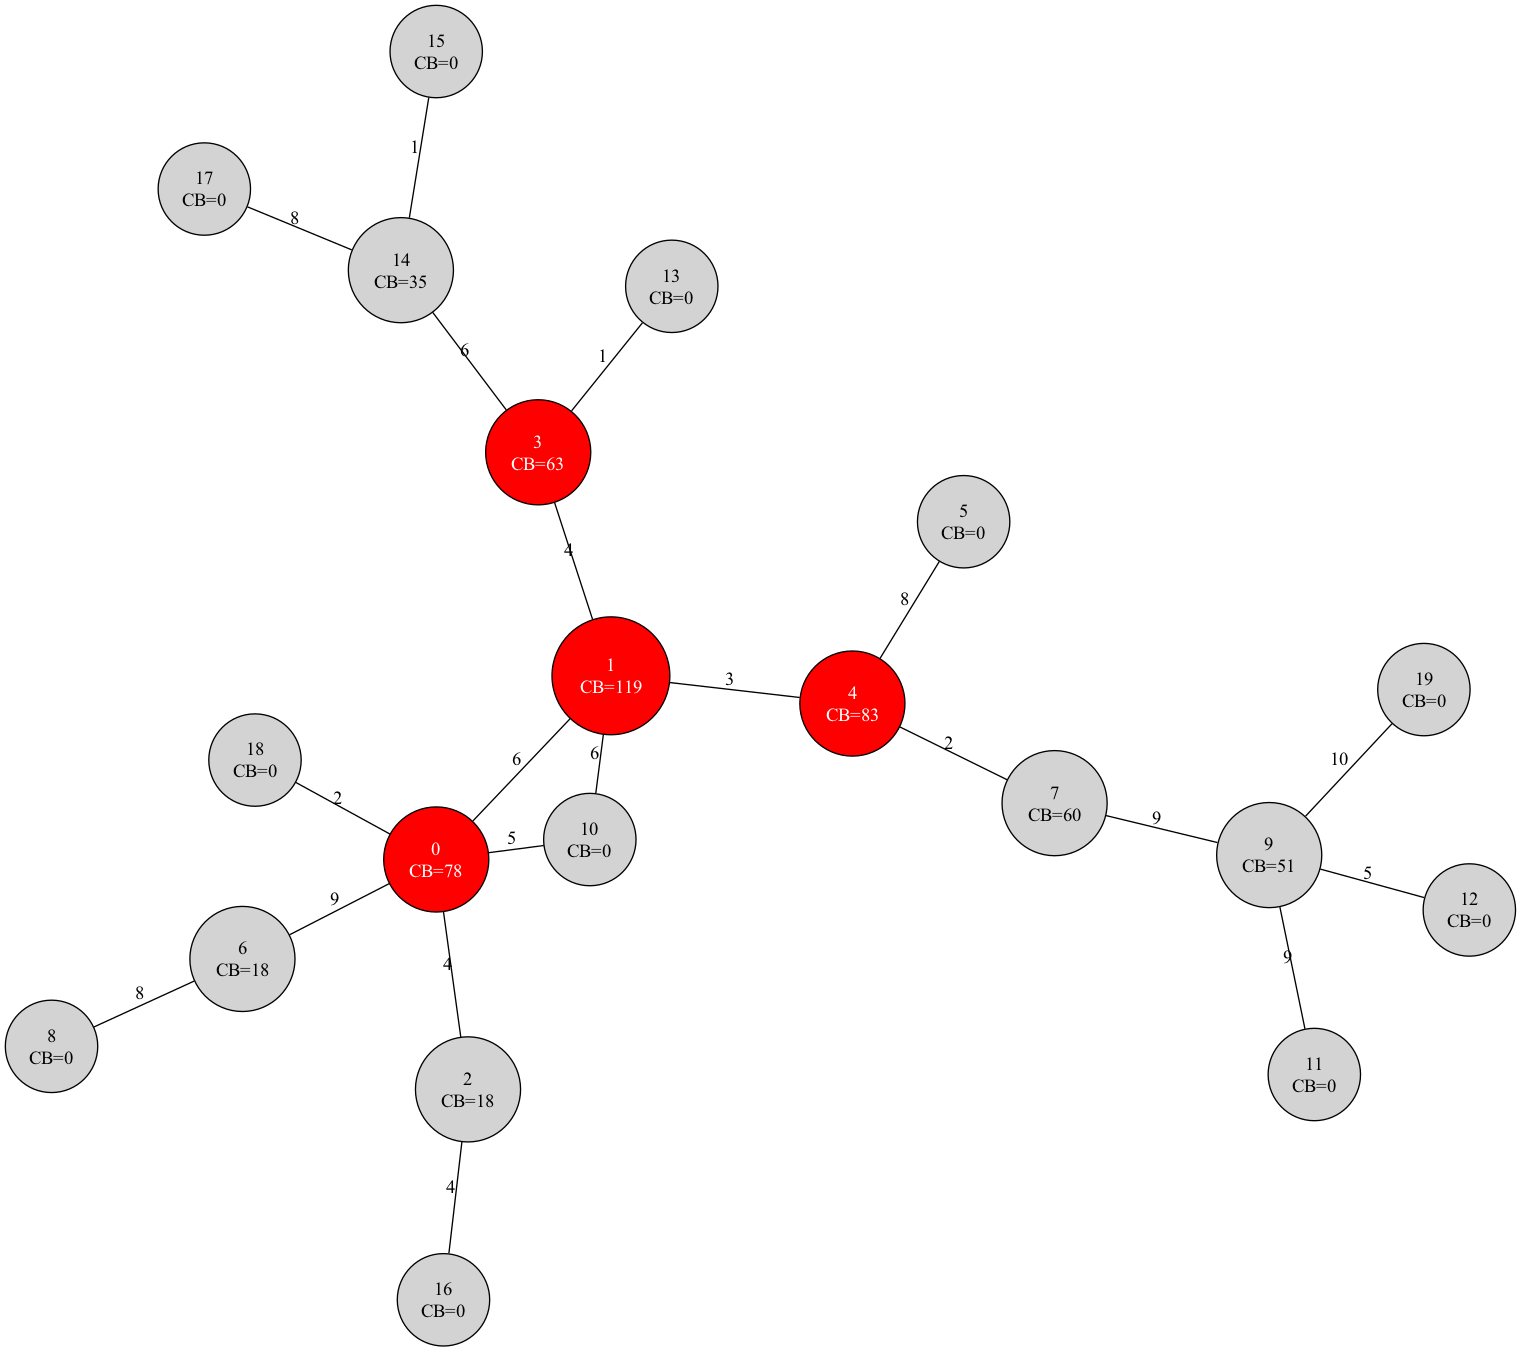
\includegraphics[width=0.7\textwidth]{grafo_w.png}
	\caption{Grafo pesato di esempio: in rosso i nodi con betweenness più alta. Le
		etichette sugli archi indicano i pesi. Rispetto al caso non pesato, i pesi
		modificano la struttura dei cammini minimi e, di conseguenza, l'insieme dei nodi
		che vi giacciono.}
	\label{fig:grafo_w}
\end{figure}


\chapter{Risultati sperimentali}

\section{Impostazione degli esperimenti}

Le prove sono state condotte generando grafi casuali connessi mediante la funzione
\texttt{genera\_grafo} descritta nel Capitolo~2. Al fine di contenere il rumore di
misura sono stati adottati i seguenti accorgimenti:
\begin{itemize}
	\item ciascuna configurazione $(n,m)$ è stata cronometrata ripetendo la misura
	      cinque volte sullo stesso grafo e assumendo il tempo \emph{minimo}: la
	      corsa più veloce è quella meno disturbata dalle interferenze del sistema
	      operativo (scheduling, altri processi), e fornisce dunque la stima più
	      pulita del costo effettivo dell'algoritmo;
	\item i tempi sono stati rilevati tramite
	      \texttt{std::chrono::high\_resolution\_clock}, cronometrando la sola
	      invocazione di \texttt{brandes};
	\item è stata anteposta una fase di \emph{warm-up} per stabilizzare la frequenza
	      del processore.
\end{itemize}
I risultati sono salvati in un file \texttt{risultati.csv} ed elaborati da uno
script Python (\texttt{plot.py}) per la produzione dei grafici; la variante pesata
segue il medesimo protocollo, con output su \texttt{risultati\_w.csv}.

\section{La pipeline sperimentale}

L'intera raccolta dei dati è automatizzata: nessun grafo viene letto da file né
prodotto a mano. Ogni eseguibile genera internamente i grafi, cronometra
l'algoritmo e scrive un file \texttt{.csv}, che uno script Python trasforma poi in
figura. Il flusso, identico per le tre varianti, si articola in cinque stadi.

\begin{enumerate}
	\item \textbf{Sweep dei parametri.} Due cicli annidati esplorano le
	      configurazioni: la densità $d$ dal $10\%$ al $90\%$ a passi del $10\%$ e
	      il numero di vertici $n$ da $100$ a $2000$ a passi di $100$. Per ciascuna
	      coppia il numero di archi è fissato a $m=\lfloor d\cdot\binom{n}{2}\rfloor$;
	      le configurazioni con $m<n-1$ (troppo pochi archi per essere connesse)
	      vengono saltate.
	\item \textbf{Generazione del grafo.} Per ogni $(n,m)$ la funzione
	      \texttt{genera\_grafo(n, m, seed)} costruisce un grafo casuale connesso
	      (spanning tree + archi aggiuntivi, Capitolo~2). Il seme è fisso, così che
	      l'esperimento sia \emph{riproducibile}: rilanciando i programmi si ottengono
	      gli stessi grafi e quindi gli stessi tempi a meno del rumore di misura.
	\item \textbf{Warm-up.} Prima del ciclo di misura l'algoritmo gira alcune volte
	      su un grafo intermedio, scartandone i risultati, per portare il processore
	      alla frequenza di regime e precaricare le cache.
	\item \textbf{Cronometraggio.} La sola chiamata a \texttt{brandes} è misurata con
	      \texttt{std::chrono}, ripetuta cinque volte; si conserva il tempo
	      \emph{minimo}, la corsa meno disturbata dal sistema operativo.
	\item \textbf{Scrittura del CSV.} Per ogni configurazione viene emessa una riga
	      \texttt{n,m,densita,tempo\_us} (tempo in microsecondi). Il file risultante è
	      l'unico ingresso degli script Python, che raggruppano le righe per densità e
	      tracciano il tempo in funzione di $n$ (o di $n\cdot m$).
\end{enumerate}

Oltre allo sweep, gli eseguibili non pesato e pesato generano un piccolo grafo di
esempio ($n=20$), ne evidenziano i nodi-ponte (primo $20\%$ per betweenness) e ne
scrivono la descrizione Graphviz (\texttt{.dot}), resa poi in immagine da
\texttt{neato} --- è l'origine delle Figure~\ref{fig:grafo} e~\ref{fig:grafo_w}.

La corrispondenza fra programma, file prodotto e figura della tesina è riassunta
nella Tabella~\ref{tab:pipeline}.

\begin{table}[H]
	\centering
	\begin{tabular}{@{}llll@{}}
		\toprule
		Programma            & Algoritmo          & File \texttt{.csv}          & Figure prodotte \\
		\midrule
		\texttt{brandes}          & Brandes (BFS)      & \texttt{risultati.csv}          & \ref{fig:tempi}, \ref{fig:confronto_dens} \\
		\texttt{brandes\_weighted} & Brandes (Dijkstra) & \texttt{risultati\_w.csv}        & \ref{fig:tempi_w} \\
		\texttt{standard}         & classico $O(n^3)$  & \texttt{risultati\_standard.csv} & \ref{fig:confronto_dens} \\
		\bottomrule
	\end{tabular}
	\caption{Pipeline: ogni eseguibile produce un CSV; gli script Python
	(\texttt{plot.py}, \texttt{confronto\_densita.py}) li combinano nelle figure.}
	\label{tab:pipeline}
\end{table}

\section{Verifica di correttezza}

Prima di procedere all'analisi dei tempi è indispensabile accertare la
correttezza dei valori calcolati dall'implementazione. I valori di $C_B$ prodotti
dal codice C++ sono stati confrontati con quelli forniti dalla funzione
\texttt{betweenness\_centrality} della libreria NetworkX~\cite{networkx}
(con \texttt{normalized=False}, così da adottare la medesima scala) su un grafo di
prova con $n=15$ e $m=20$.

\begin{table}[H]
	\centering
	\caption{Confronto $C_B$: implementazione C++ vs NetworkX (estratto).}
	\begin{tabular}{rrrr}
		\toprule
		nodo & C++     & NetworkX & differenza          \\
		\midrule
		1    & 36.3333 & 36.3333  & $3.3\times10^{-11}$ \\
		3    & 36.3333 & 36.3333  & $3.3\times10^{-11}$ \\
		0    & 33.6667 & 33.6667  & $3.3\times10^{-11}$ \\
		5    & 16.3333 & 16.3333  & $3.3\times10^{-11}$ \\
		11   & 0.0000  & 0.0000   & $0.0$               \\
		13   & 0.3333  & 0.3333   & $3.3\times10^{-13}$ \\
		\bottomrule
	\end{tabular}
\end{table}

La differenza massima riscontrata sull'insieme dei nodi è dell'ordine di
$10^{-11}$, riconducibile al solo rumore in virgola mobile: le due implementazioni
producono il medesimo risultato. La verifica è stata ripetuta sulla versione
ottimizzata del codice (buffer riutilizzati, predecessori ricalcolati), con esito
parimenti coincidente, a conferma del fatto che le ottimizzazioni implementative non
ne alterano la correttezza.

\section{Interpretazione visiva della betweenness}

Allo scopo di attribuire un significato intuitivo alla misura, la
Figura~\ref{fig:grafo} mostra un grafo di esempio in cui i nodi con betweenness
più elevata --- i cosiddetti \emph{ponti} --- sono evidenziati in rosso.

\begin{figure}[H]
	\centering
	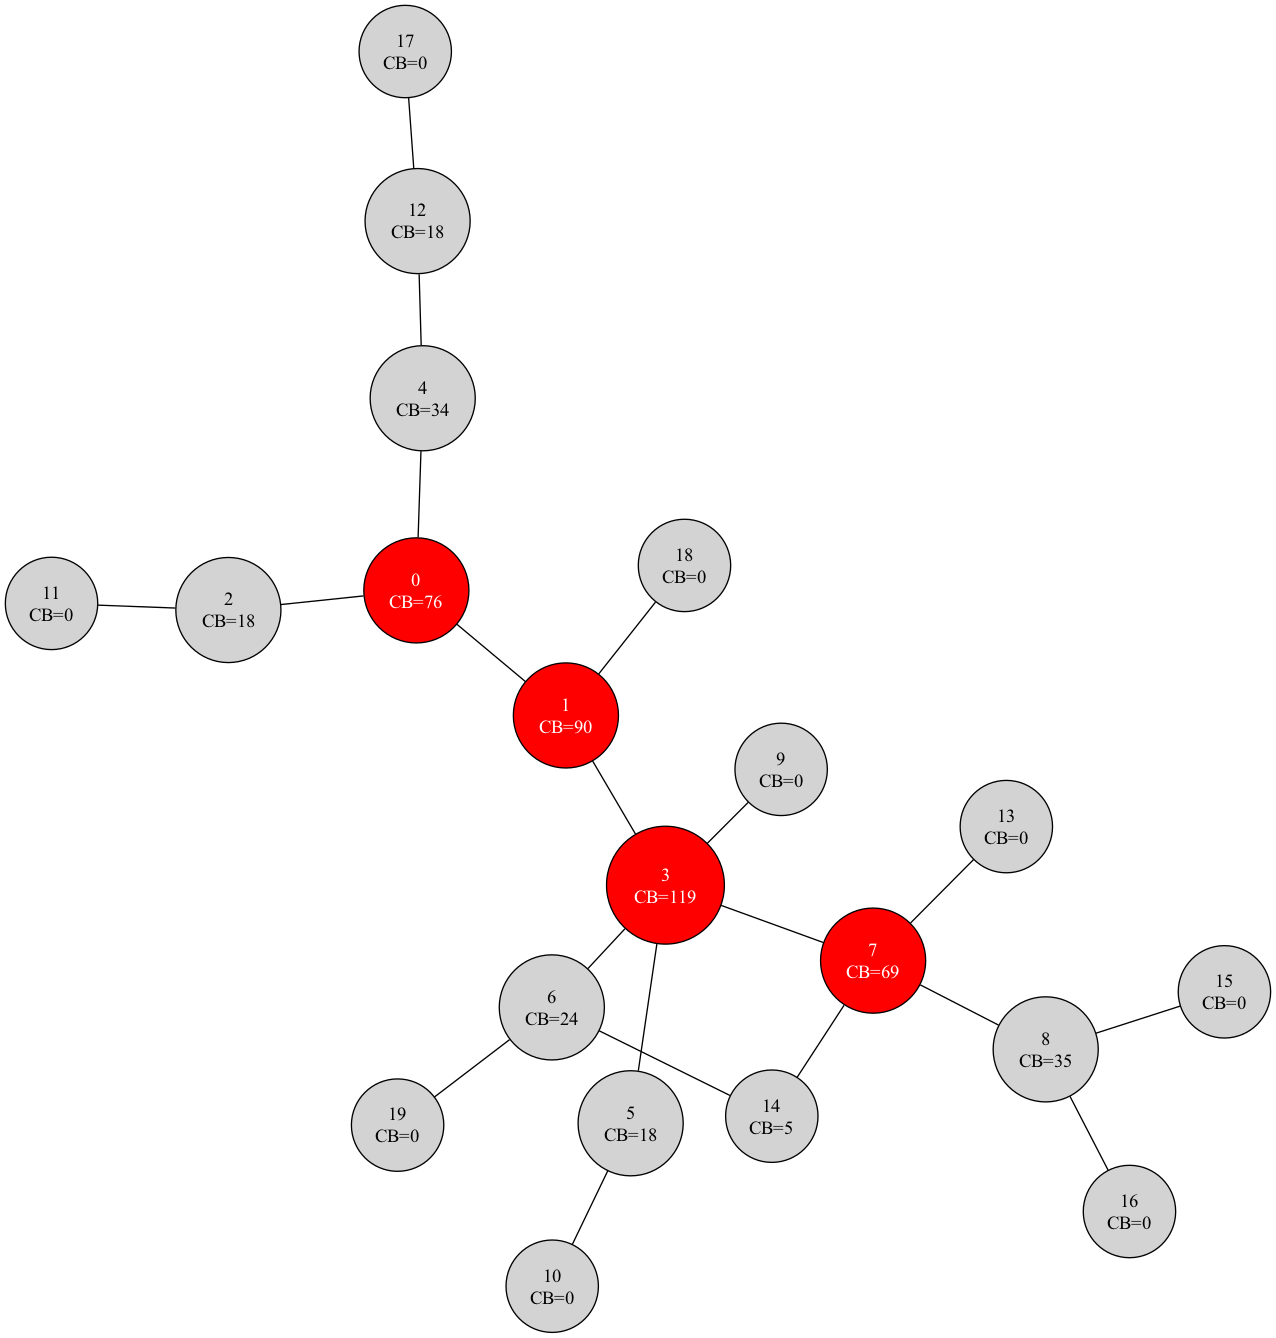
\includegraphics[width=0.7\textwidth]{grafo.png}
	\caption{Grafo di esempio: in rosso i nodi con betweenness più alta. Si nota come
		i ponti non siano necessariamente i nodi con più connessioni, ma quelli che
		giacciono sui passaggi obbligati tra le diverse zone del grafo. I nodi foglia,
		come il nodo 11, hanno betweenness nulla.}
	\label{fig:grafo}
\end{figure}


\section{Analisi della complessità}

Per verificare la complessità $O(nm)$ è stato misurato il tempo di esecuzione al
variare di $n$ e $m$. Riportando il tempo in funzione del prodotto $n\cdot m$ si
ottiene un andamento sostanzialmente lineare, con coefficiente di determinazione
$R^2\approx 0.93$. Una rappresentazione
complementare, con il tempo in funzione di $n$ per densità fissata, è riportata
nella Figura~\ref{fig:tempi} della sezione successiva.

\subsection{Il sovraccarico lineare per sorgente}

Un'osservazione rilevante emersa dagli esperimenti riguarda il comportamento a
$m$ fissato: mantenendo costante il numero di archi e incrementando $n$, il tempo
non cresce in modo lineare bensì quadratico. La causa risiede nel fatto che il
costo effettivo per ciascuna sorgente non è $O(m)$ ma $O(n+m)$, poiché
l'inizializzazione dei buffer (\texttt{d}, \texttt{sigma}, \texttt{delta})
richiede $O(n)$ operazioni a ogni sorgente. Il costo complessivo è dunque
\begin{equation}
	O\bigl(n\cdot(n+m)\bigr) = O(n^2 + nm),
\end{equation}
e quando $m$ è piccolo rispetto a $n$ il termine $n^2$ risulta dominante. Ciò
giustifica la curvatura osservata e mette in evidenza come la stima $O(nm)$
presupponga implicitamente grafi sufficientemente densi ($m\gtrsim n$).

\section{Riproduzione dell'esperimento di Brandes}

Infine, è stato riprodotto lo schema sperimentale dell'articolo originale: uno
sweep del numero di vertici da $100$ a $2000$, con una curva per ciascuna densità
compresa tra il $10\%$ e il $90\%$, secondo lo stesso impianto della Figura~3 di
Brandes~\cite{brandes2001}. Il risultato è riportato nella
Figura~\ref{fig:tempi}.

\begin{figure}[H]
	\centering
	
\includegraphics[width=0.8\textwidth]{brandes_plot.png}
	\caption{Tempo di esecuzione (caso non pesato) in funzione del numero di
		vertici, una curva per ciascuna densità dal $10\%$ al $90\%$: riproduzione
		della Figura~3 dell'articolo originale di Brandes.}
	\label{fig:tempi}
\end{figure}

La rappresentazione per densità non è una semplice scelta estetica: ciascuna curva
fissa la densità, ossia un valore di $m$ proporzionale a $n^2$, e isola così
l'effetto del numero di archi sul tempo. A parità di $n$, passando da una curva
all'altra cambia esclusivamente $m$; lo scostamento verticale fra le curve misura
perciò in modo diretto la dipendenza da $m$ insita nel fattore $O(nm)$. Si osserva
infatti che, fissato $n$, il tempo cresce con la densità per gran parte
dell'intervallo, come atteso da una complessità lineare in $m$.

Alle densità più elevate, però, l'andamento si inverte e il tempo torna a
diminuire pur continuando $m$ a crescere. Il fenomeno è sistematico --- si ripresenta
identico a $n=1000$ e $n=2000$ --- e ha una spiegazione strutturale: nei grafi quasi
completi il diametro si riduce a $1$--$2$ e quasi tutti i vertici giacciono a
distanza unitaria dalla sorgente. Di conseguenza pochissimi archi soddisfano la
condizione di cammino minimo $d_w = d_v+1$, e crollano sia gli aggiornamenti del
conteggio $\sigma$ sia, soprattutto, gli accumuli di dipendenza $\delta$, che
costituiscono le operazioni aritmeticamente più onerose. Il numero di archi
\emph{esaminati} resta $\Theta(nm)$, ma il lavoro \emph{effettivo} per arco diventa
quasi nullo, e il tempo cala. Le curve, dunque, non si limitano a confermare
l'andamento teorico: rendono evidente che il costo dipende dalla \emph{struttura}
dei cammini minimi e non dal solo numero di archi, motivo per cui la densità è il
parametro più significativo da fare variare.

\section{Confronto sperimentale con l'approccio standard}

L'analisi precedente riguarda il solo algoritmo di Brandes; per quantificarne il
vantaggio è stato affiancato, sui medesimi grafi, l'approccio standard $O(n^3)$
descritto nel Capitolo~1. La Figura~\ref{fig:confronto_dens} riporta, per ciascuna
densità, le due curve sovrapposte in funzione di $n$ sul range comune (fino a
$n=1000$, oltre il quale l'$O(n^3)$ diventa proibitivo sia per il tempo sia per la
memoria $O(n^2)$). La scelta di confrontare \emph{a parità di densità} è proprio ciò
che rende leggibile il risultato: è la densità a determinare il regime in cui ci si
trova.

\begin{figure}[H]
	\centering
	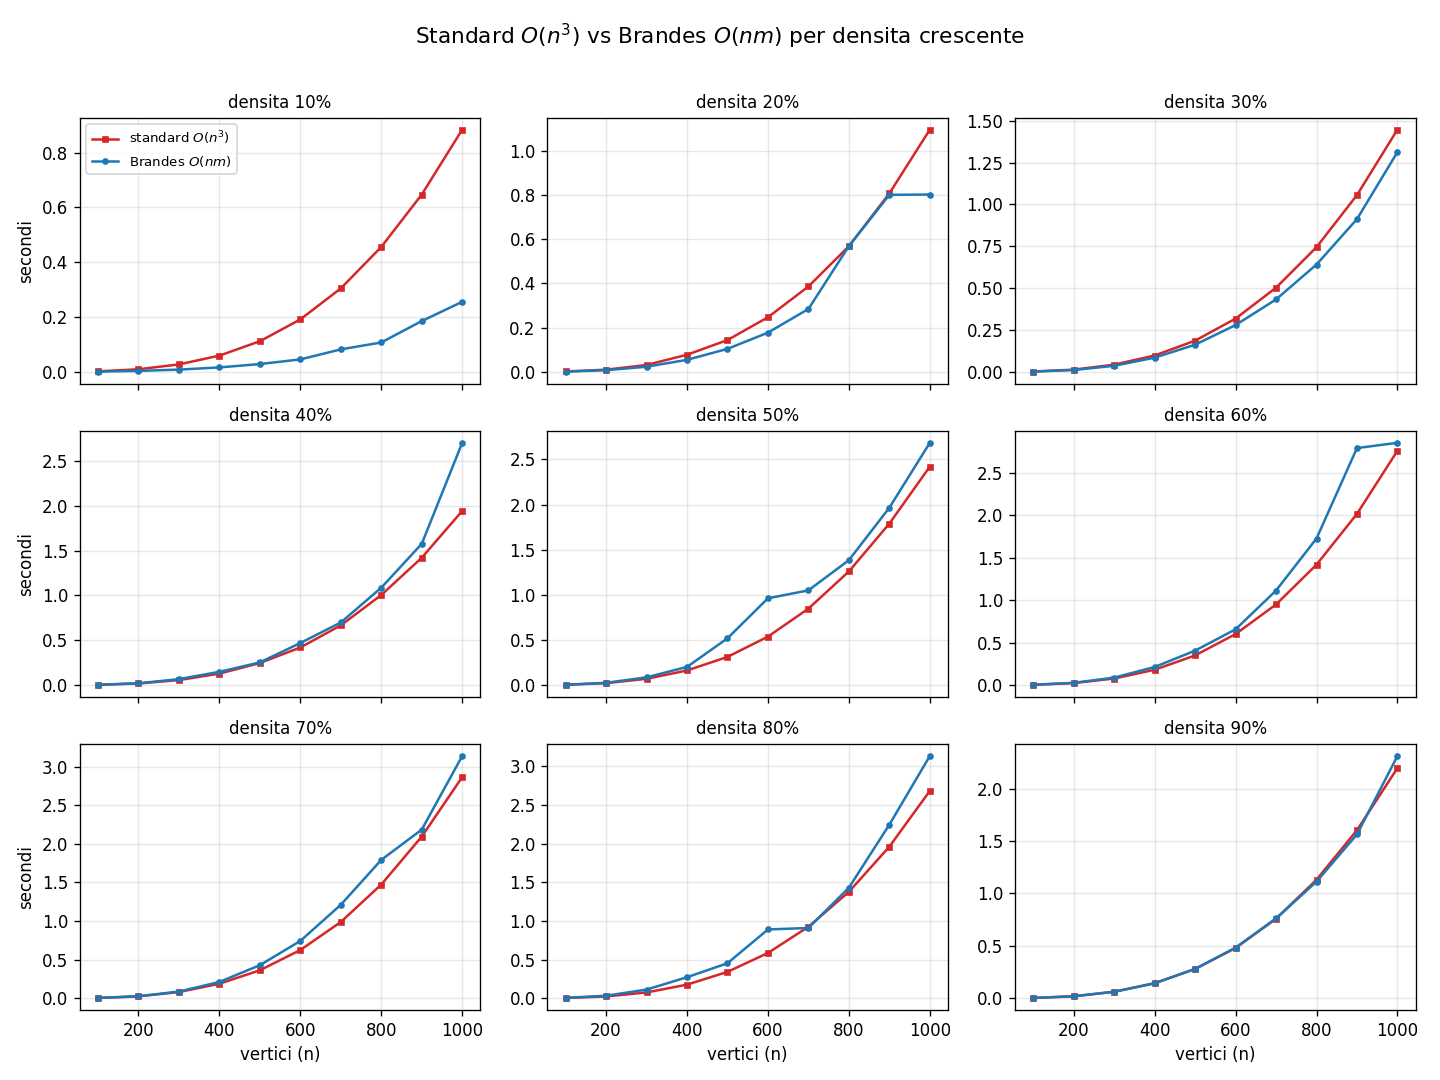
\includegraphics[width=\textwidth]{confronto_densita.png}
	\caption{Confronto fra l'approccio standard $O(n^3)$ (rosso) e l'algoritmo di
		Brandes $O(nm)$ (blu) in funzione di $n$, un pannello per ciascuna densità dal
		$10\%$ al $90\%$. Alle basse densità Brandes è nettamente più rapido; al crescere
		della densità le due curve diventano dello stesso ordine di grandezza.}
	\label{fig:confronto_dens}
\end{figure}

Il confronto chiarisce il ruolo della densità. L'approccio standard è dominato dal
triplo ciclo sulle coppie, di costo $\Theta(n^3)$ \emph{a prescindere} dal numero
di archi; il suo tempo varia perciò poco con la densità. La lieve diminuzione che
si osserva alle densità più alte è imputabile alla seconda fase: nei grafi quasi
completi i cammini minimi sono brevissimi e il criterio di Bellman è soddisfatto da
pochi vertici intermedi, riducendo le operazioni di accumulo.

L'algoritmo di Brandes, di costo $O(nm)$, dipende invece direttamente da $m$. Nei
grafi \emph{sparsi} (densità $10$--$30\%$) il numero di archi è ridotto ed esso
risulta nettamente più veloce: a $n=1000$ il vantaggio raggiunge un fattore
prossimo a $3$. Al crescere della densità $m$ tende a $\Theta(n^2)$ e il costo
$O(nm)$ degenera a $O(n^3)$: nelle densità intermedie e alte le due curve si
intrecciano e restano dello stesso ordine di grandezza. Alle densità più estreme,
anzi, entrambe tornano ad accelerare per il medesimo motivo strutturale già
richiamato --- la quasi-completezza del grafo rende i cammini minimi triviali e
riduce drasticamente le operazioni di accumulo in entrambi gli algoritmi --- come
discusso a proposito della Figura~\ref{fig:tempi}. Il vantaggio robusto di Brandes va
dunque cercato nei grafi sparsi --- quelli tipici delle reti reali --- e,
soprattutto, nello \emph{spazio}: $O(n+m)$ lineare contro l'$O(n^2)$ dello standard,
a qualunque densità.


\chapter{Conclusioni}

\section{Sintesi del lavoro}

In questa tesina è stato implementato in C++ l'algoritmo di Brandes per il
calcolo della betweenness centrality su grafi non orientati, nelle due varianti
\emph{non pesata} (BFS) e \emph{pesata} (Dijkstra). Il
lavoro ha riguardato quattro aspetti complementari:
\begin{itemize}
	\item \textbf{correttezza}: i valori prodotti coincidono con quelli della
	      libreria di riferimento NetworkX a meno del rumore in virgola mobile
	      ($\sim 10^{-11}$), sia nella versione base sia in quella ottimizzata,
	      e anche nella variante pesata (confronto con \texttt{weight='weight'});
	\item \textbf{efficienza}: l'analisi sperimentale conferma la complessità
	      $O(nm)$ prevista dalla teoria per il caso non pesato, evidenziando
	      inoltre il sovraccarico lineare per sorgente che conduce al costo
	      complessivo $O(n^2+nm)$;
	\item \textbf{estensione ai grafi pesati}: la sostituzione della BFS con
	      l'algoritmo di Dijkstra e una coda a priorità consente di
	      trattare archi con peso arbitrario, a fronte di un fattore logaritmico
	      aggiuntivo ($O(nm\log n)$ con heap binario), come confermato dai tempi
	      misurati al variare della densità;
	\item \textbf{ottimizzazione}: il riutilizzo dei buffer di memoria e
	      l'eliminazione delle liste di predecessori riducono la costante
	      moltiplicativa senza modificare la complessità asintotica né i risultati.
\end{itemize}

In conclusione, l'algoritmo di Brandes si conferma una soluzione elegante ed
efficiente al problema della betweenness centrality: il passaggio da uno spazio
$O(n^2)$ a uno spazio lineare $O(n+m)$, ottenuto grazie all'accumulo ricorsivo
delle dipendenze, è ciò che ne rende possibile l'uso su reti di grande
dimensione.


\begin{thebibliography}{9}
	\bibitem{brandes2001} U.~Brandes,
	\emph{A Faster Algorithm for Betweenness Centrality},
	Journal of Mathematical Sociology, 25(2):163--177, 2001.
	\bibitem{freeman1977} L.~C.~Freeman,
	\emph{A Set of Measures of Centrality Based on Betweenness},
	Sociometry, 40(1):35--41, 1977.
	\bibitem{anthonisse1971} J.~M.~Anthonisse,
	\emph{The Rush in a Directed Graph},
	Stichting Mathematisch Centrum, Amsterdam, 1971.
	\bibitem{fredman1987} M.~L.~Fredman, R.~E.~Tarjan,
	\emph{Fibonacci Heaps and Their Uses in Improved Network Optimization Algorithms},
	Journal of the ACM, 34(3):596--615, 1987.
	\bibitem{networkx} A.~Hagberg, D.~Schult, P.~Swart,
	\emph{Exploring Network Structure, Dynamics, and Function using NetworkX},
	Proceedings of the 7th Python in Science Conference, 2008.
\end{thebibliography}

\end{document}
